\chapter{Harmonogram realizacji projektu}
\label{cha:harmonogram}

\section{Diagram Ganta pracy}

Na \figurename~\ref{fig6} przedstawiono diagram, zawierający informacje o kolejności podejmowanych działań oraz ich długości pracy.
Diagram utworzony został przy użyciu \url{https://www.drawio.com/}.
\begin{figure}[H]
    \centering
    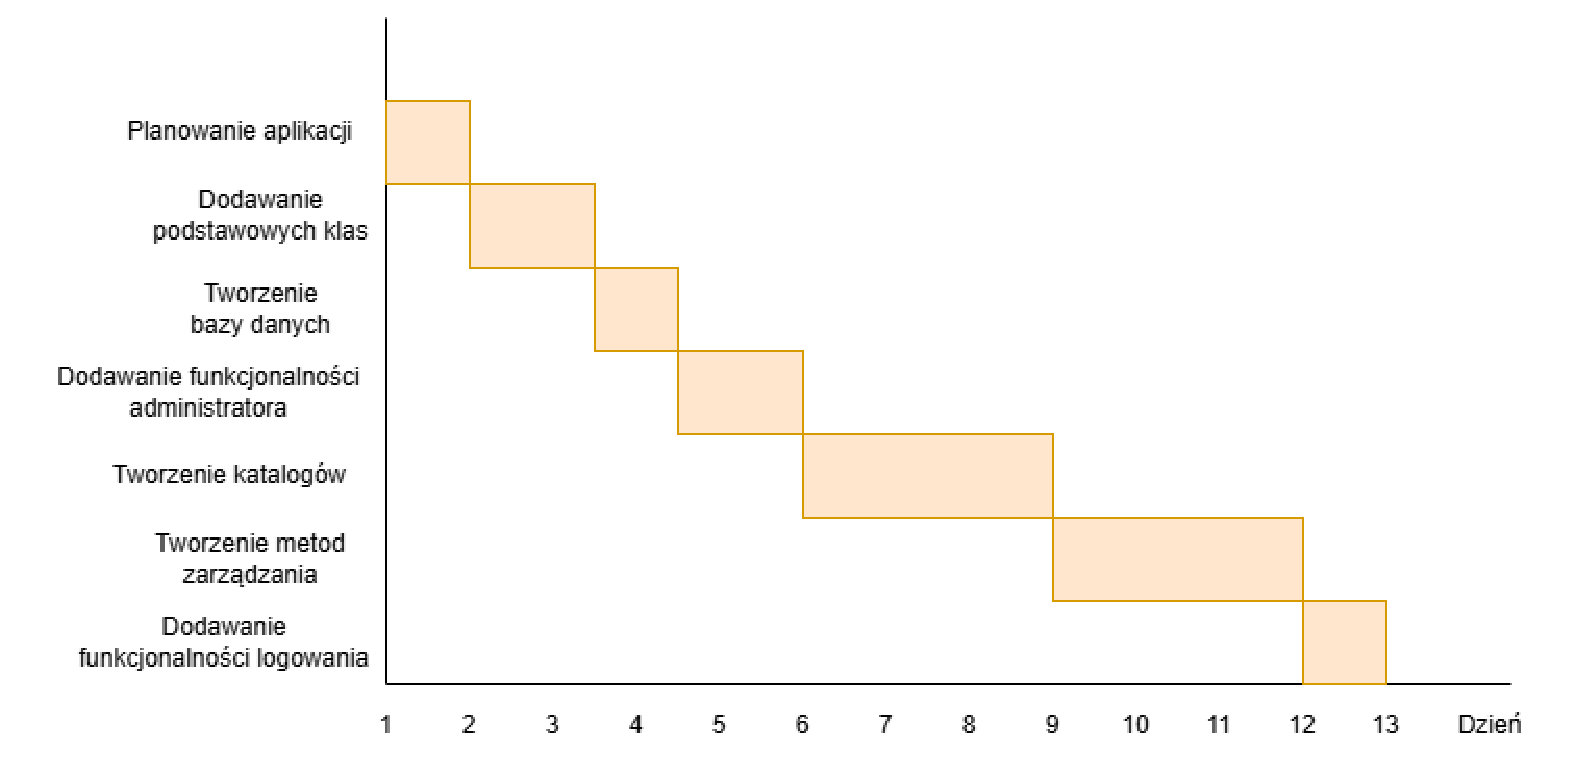
\includegraphics[width=\linewidth]{figures/fig_0006.eps}\\
    \caption{Diagram Ganta pracy.\label{fig6}}
\end{figure}

Najbardziej wymagającą i czasochłonną częścią prac okazuje się być zrealizowanie funkcjonalnych, przystępnych i estetycznych wizualnie 
katalogów produktów, zamówień i użytkowników.

\section{Repozytorium i system kontroli wersji}
Całość projektu wraz z wyeksportowaną bazą danych zostały przeniesione do repozytorium GitHub \url{https://github.com/Buczul/Symulator_sklepu_internetowego_repo}.